\documentclass[12pt,a4paper]{article}

\usepackage[croatian]{babel}
\usepackage[utf8]{inputenc}
\usepackage[hyphens]{url}

\usepackage{listings}

\usepackage{color}
 
\definecolor{codegreen}{rgb}{0,0.6,0}
\definecolor{codegray}{rgb}{0.5,0.5,0.5}
\definecolor{codepurple}{rgb}{0.58,0,0.82}
\definecolor{backcolour}{rgb}{0.95,0.95,0.92}
 
\lstdefinestyle{Python}{
    backgroundcolor=\color{backcolour},   
    commentstyle=\color{codegreen},
    keywordstyle=\color{magenta},
    numberstyle=\tiny\color{codegray},
    stringstyle=\color{codepurple},
    basicstyle=\footnotesize,
    breakatwhitespace=false,         
    breaklines=true,                 
    captionpos=b,                    
    keepspaces=true,                 
    numbers=left,                    
    numbersep=5pt,                  
    showspaces=false,                
    showstringspaces=false,
    showtabs=false,                  
    tabsize=2
}

\lstdefinestyle{Bash}{
	backgroundcolor=\color{backcolour},
	basicstyle=\ttfamily,
  	showstringspaces=false,
  	commentstyle=\color{red},
  	keywordstyle=\color{blue}
}

\usepackage{graphicx}

\usepackage[margin=2cm]{geometry}
\usepackage[colorlinks=true,urlcolor=black]{hyperref}
\pagenumbering{arabic}


\begin{document}
	\title{Očitavanje senzorskih podataka korištenjem računala Raspberry Pi 3}


	\date{9. svibnja 2017.}
	\author{Autor: \\ Leonard Volarić Horvat \\ \\ Mentori: \\ Nenad Katanić, mag. ing.\\
Doc. dr. sc. Boris Milašinović}
	\maketitle

	\tableofcontents
	\newpage

\section{Uvod}
Ovaj će seminarski rad obraditi problematiku korištenja računala Raspberry Pi 3 za prikupljanje podataka sa senzora. Ukratko će se opisati sklopovska arhitektura računala Raspberry Pi 3 te pripadajuća programska podrška, uz nekoliko primjera korištenja. \\ \par
Kao vrlo pristupačno malo računalo, Raspberry Pi je vrlo popularan kao ugradbeno računalo, a budući da ugradbena računala vrlo često za svoj rad koriste raznolike senzore, za ovaj će rad biti ključno razumjeti osnovne principe povezivanja senzora i računala, uzimajući u obzir sklopovski i programski aspekt. Shodno tome, bit će izložen kratak opis jednog akcelerometra, u funkciji senzora za mjerenje vibracija, te jednog mikrofona, poglavito u funkciji senzora glasnoće. \\ \par
Ukratko će se opisati neke od dostupnih biblioteka i programskih okvira namijenjenih za rad sa senzorima, s naglaskom na već spomenute akcelerometre i mikrofone. Konačno, bit će pokazan i jednostavan primjer programskog koda za očitavanje podataka sa senzora uz prateći primjer vizualnog prikaza senzorskih podataka. \\
\newpage


\section{Raspberry Pi}

Raspberry Pi je serija malih računala razvijanih od strane zaklade Raspberry Pi Foundation. Odlikuju ih niska cijena, dobre performanse s obzirom na cijenu, pristupačnost i lako korištenje te male fizičke dimenzije. Programska je podrška otvorena i vrlo dobro dokumentirana, a zajednica ljudi koji koriste Raspberry Pi je velika, pristupačna i konstruktivna. \\
\par
U trenutku pisanja su dostupni Raspberry Pi 1, 2 i 3, te minijaturni Raspberry Pi Zero. U nastavku će rada riječ biti o Raspberry Pi 3 inačici, koja se vidi na Slici \ref{fig:rpi3}, a bit će oslovljena kao "RPi3".
\begin{figure}[h!]
  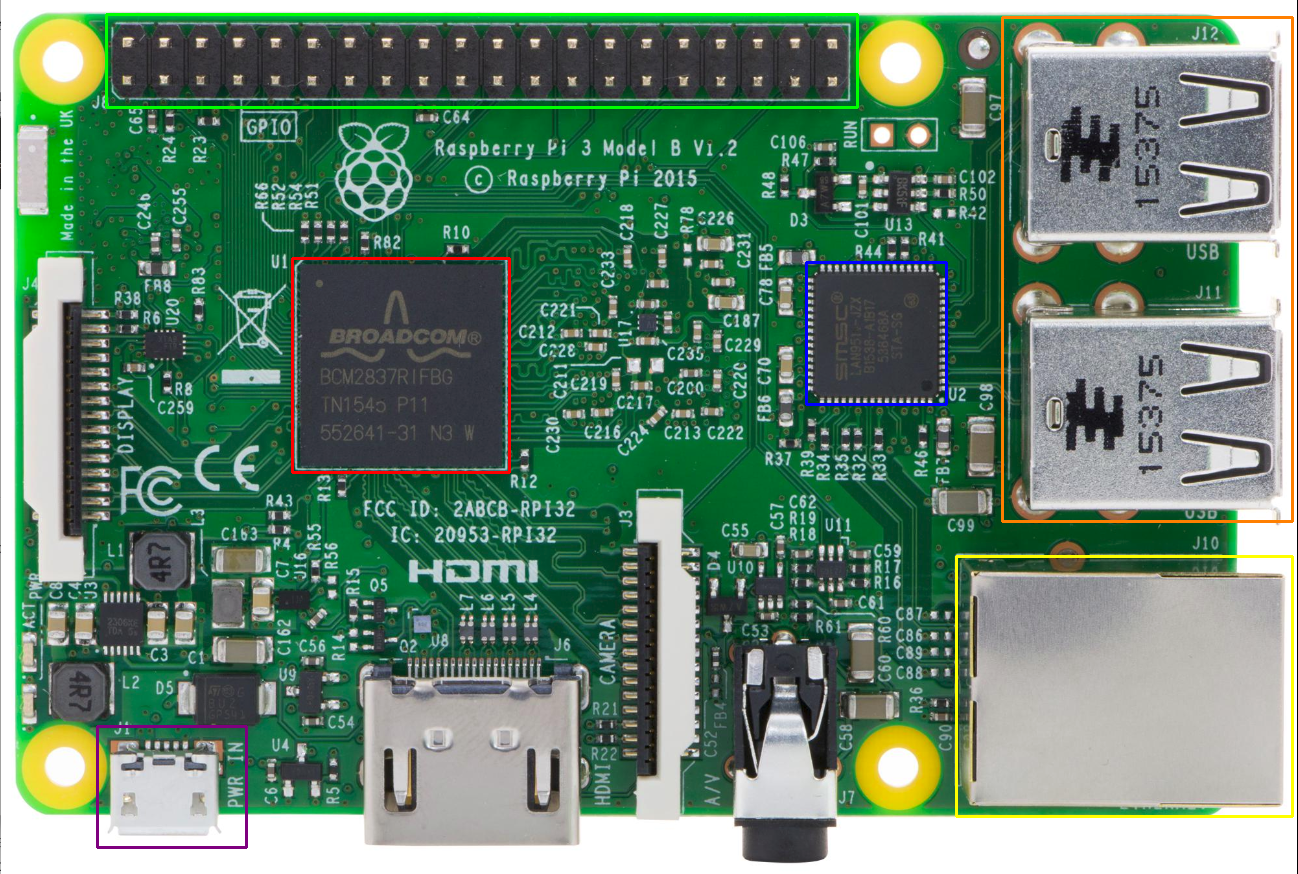
\includegraphics[width=\linewidth]{slike/rpi3_color.png}
  \caption{Raspberry Pi 3B.}
  \label{fig:rpi3}
\end{figure}

	\subsection{Sklopovlje}
		\paragraph{\underline{Glavni čipovi}} % (fold)
		\label{par:main_chips}
		
		Glavne procesne jedinice nalaze se u čipu Broadcom BCM2837, koji je na slici označen crvenim pravokutnikom. Riječ je o tzv. \textit{System-on-Chip} (SoC) čipu koji sadrži:
		\begin{itemize}
			\item \textbf{CPU} - 64-bitni ARMv8 Cortex A53 s četiri jezgre na 1.2 GHz,
			\item \textbf{GPU} - VideoCore IV na 400 MHz.
		\end{itemize}

		\par Taj je SoC spregnut s \textbf{radnom memorijom} s druge strane tiskane pločice. Riječ je o LPDDR2 SDRAM memoriji, s kapacitetom od 1 GB.

		\par Za bežičnu je komunikaciju zadužen procesor osnovnog pojasa (engl. \textit{baseband processor}) BCM43438, također od tvrtke Broadcom, koji podržava WiFi i Bluetooth 4.1 protokole. Smješten je na stražnjoj strani pločice, a spregnut je s antenom na prednjoj strani. Nije zgorega napomenuti da je Raspberry Pi 3 prva inačica ovog računala koja ima ugrađeno sklopovlje za bežičnu komunikaciju.

		\par Konačno, SMSC LAN9514 (na slici uokviren plavom bojom) vrši funkciju USB čvora i Ethernet upravljača. Povezan je s procesorom jednom USB vezom, pa sa svakim od četiri USB priključka, te s Ethernet priključkom procesor komunicira preko te USB veze.
		% paragraph glavni_cipovi (end)

		\paragraph{\underline{Ulazno-izlazni priključci}} % (fold)
		\label{par:IO_ports}
		
		Kao i svako drugo računalo, i RPi3 bi bio prilično beskoristan bez mogućnosti komunikacije s vanjskim svijetom. Naravno, na njemu postoji mnoštvo ulazno-izlaznih sučelja, a način na koji su ona izvedena je uvelike zaslužan za takvu popularnost ovog računala. Za ovaj seminar najvažniji priključci označeni su na Slici \ref{fig:rpi3}, a u nastavku je dan pregled tih sučelja:
		\begin{itemize}
			\item Četiri \textbf{USB 2.0} priključka [narančasti pravokutnik]
			\item Jedan \textbf{Ethernet} priključak [žuti pravokutnik]
			\item Jedan \textbf{microUSB} priključak - samo za napajanje, ne i za komunikaciju [ljubičasti pravokutnik]
			\item Četrdeset ulazno-izlaznih pinova opće namjene (\textbf{GPIO} - \textit{General Purpose Input/Output}) [zeleni pravokutnik]
			\item Ulaz za \textbf{\textit{microSD} karticu} (s druge strane pločice)
			\item Audio priključak i HDMI izlaz
			\item Poseban priključak za službenu Raspberry Pi kameru
			\item Poseban \textit{display} priključak
		\end{itemize}

		\par Od posebne su važnosti za ovaj rad GPIO pinovi. Oni, su, naime, ključni za komunikaciju sa senzorima koji će biti razmotreni kasnije u radu. Omogućuju najčešće korištene \textit{low-level} protokole za sklopovsku komunikaciju: \textbf{I$^2$C, TTL i SPI.} Naravno, sadrže i pinove za napajanje i uzemljenje sklopova, kao i pinove namijenjene za korisničku definiciju ponašanja.
		% paragraph ulazno_izlazni_priključci (end)

	\subsection{Programska podrška}
		Programska je podrška za RPi3, baš kao i sklopovlje, izvedena s ciljem jednostavnosti i fleksibilnosti korištenja. Budući da nije riječ o mikrokontroleru (poput, primjerice, popularnog Arduina), već o potpuno opremljenom računalu, očito je da RPi3 mora imati neki operacijski sustav (u nastavku: OS). On se u glavnini slučajeva nalazi na \textbf{\textit{microSD} kartici}, koja ima ulogu sekundarne memorije.\footnote{Moguće je pokrenuti OS i s, primjerice, nekog USB tvrdog diska, ali to nadilazi temu ovog seminara.} Ovdje kao najpopularniji OS za RPi u priču ulazi \textbf{Raspbian.} \\

		\par Raspbian je besplatan i otvoren operacijski sustav baziran na distribuciji Linuxa zvanoj "Debian". Ono zbog čega je Raspbian toliko popularan jest činjenica da je taj \textbf{OS optimiziran upravo za Raspberry Pi sklopovlje.}\footnote{Ovo se može zaključiti i iz imena distribucije, koje je \textit{portmanteau} pojmova "Raspberry Pi" i "Debian".} Drugim riječima, Raspbian je distribucija Linuxa koja:
		\begin{itemize}
			\item je vrlo jednostavna za instalaciju i dolazi potpuno opremljena za normalan računalni rad - uključujući i \textbf{grafičko korisničko sučelje} (\textit{GUI - Graphical User Interface}) 
			\item dolazi s već instaliranom programskom podrškom za komunikaciju sa specijaliziranim sklopovljem (poput GPIO pinova) - primjerice, \textbf{iz terminala, C-a ili Pythona.}
		\end{itemize}


	\subsection{Primjeri korištenja}
	Uzevši u obzir ranije spomenute prednosti RPi3 računala - cijena, pristupačnost i dimenzije - RPi računala najčešće nađu svoju primjenu u dva konteksta:
	\begin{itemize}
		\item u edukativnim projektima (pristupačnost i cijena)
		\item u ugradbenim sustavima (male dimenzije i cijena)
	\end{itemize}
	U nastavku su ukratko izložena dva primjera korištenja RPi3 računala. Primjeri su relativno jednostavni, ali dobro ilustriraju moguće koncepte korištenja tog računala.
	\\
	\paragraph{\underline{Pametna brava}} % (fold)
	\label{par:smart_lock}
		Pametne su brave koncept novijeg datuma, a označavaju autorizaciju ulaza osobe u neki prostor, i to ne koristeći (samo) klasični, mehanički ključ, nego korištenje kartica, lozinki, ili čak, primjerice, prepoznavanja lica. Za implementaciju jedne takve brave može poslužiti bilo kakav mikrokontroler, i RPi3 bi svakako bio pretjeran za tako jednostavan zadatak, ali ono što bi moglo umanjiti taj \textit{overhead} jest, primjerice, praćenje pristupa prostoru pomoću logova, udaljeno upravljanje bravom, ili agregiranje više neovisnih zadataka slične složenosti na jednom RPi-ju.
		\par Računarska sekcija Kluba studenata elektrotehnike konkretno koristi Raspberry Pi 3 za agregiranje informacija o radu nekoliko servera, a u planu je spajanje NFC čitača (\textit{Near-Field Communication} - tehnologija beskontaktne komunikacije korištena u studentskim iskaznicama i bankovnim karticama) na taj isti RPi3, kako bi se na taj način autenticiralo osobe koje žele ući u sekciju.

	% paragraph smart_lock (end)

	\paragraph{\underline{Kućni VPN i WiFi pristupna točka}} % (fold)
	\label{par:home_vpn}
		U kontekstu komunikacijskih mreža, VPN (\textit{Virtual Private Network}) je protokol spajanja na mrežu koji omogućuje virtualno pristupanje mreži s drugog mjesta i prosljeđivanje svòg lokalnog prometa kroz taj "tunel" na način koji osigurava privatnost i sigurnost, kao i (do neke mjere) svojstva mreže (dozvole i zabrane, primjerice, ili simulacija lokalnog pristupa) kakva su na udaljenoj mreži na koju je korisnik VPN-om spojen. Implementacijski detalji VPN-a nipošto nisu trivijalni, i neće se dalje razmatrati u ovom radu, ali takav se sustav relativno bezbolno može upogoniti upravo koristeći Raspberry Pi, umjesto da se (samo?) za taj zadatak koristi neko (red veličine skuplje) računalo opće namjene.
		\par Još jedna zanimljiva mogućnost koju pruža RPi3 (ali ne i ranije inačice - barem ne bez dodatnog sklopovlja) jest postavljanje pristupne točke za WiFi, koja bi bežični promet prosljeđivala žičnoj Ethernet vezi. Tako se može, u nedostatku kompletnijeg i trajnijeg rješenja, ostvariti \textit{ad hoc} bežična mreža ili pojačivač signala.

	% paragraph home_vpn (end)

\newpage


\section{Senzori}
	Sada kada je definirano računalo koje će agregirati i analizirati očitanja senzora koje ćemo koristiti, vrijeme je da i o njima nešto rečemo. Slučaj koji promatramo jest \textbf{mjerenje vibracija} na mirnim površinama poput vrata, sa svrhom utvrđivanja \textbf{izvora} vibracija. Shodno tome, slijede kratki pregledi jednog akcelerometra - senzora za mjerenje relativnog ubrzanja - te jednog senzora glasnoće.
	Ipak, prije toga, radi lakšeg razumijevanja slijedi vrlo kratki opis dva ranije spomenuta \textit{low-level} komunikacijska protokola.

	\subsection{Komunikacijski protokoli}
	\paragraph{\underline{I$^2$C}} % (fold)
	\label{par:i2c}
		I$^2$C (engl. \textit{Inter-Integrated Circuit}) komunikacija je protokol za sinkronu serijsku komunikaciju. Odlikuje ga iznimna jednostavnost korištenja - za upogoniti I$^2$C komunikaciju potrebna su samo dva pina:
		\begin{itemize} 
			\item \textbf{SDA} (\textit{Serial DAta line}) - podatkovna linija
			\item \textbf{SCL} (\textit{Serial CLock}) - linija sa signalom takta, za sinkronizaciju.
		\end{itemize}
		Protokol omogućuje spajanje više uređaja s I$^2$C mogućnosti na istu sabirnicu, što znači da postoji i koncept adresiranja, kao i \textit{master-slave} arhitekture. Detalji implementacije toga su preširoki za ovaj rad, ali ukratko - svaki I$^2$C uređaj mora imati svoju, na sabirnici jedinstvenu adresu, koja se obično sastoji od dvije heksadekadske znamenke. 
		Ono što je jednostavnost uporabe žrtvovala jest mogućnost istovremene dvosmjerne (engl. \textit{full duplex}) komunikacije - budući da postoji samo jedna podatkovna linija, očito je da je to nemoguće, već je moguća samo \textbf{naizmjenična dvosmjerna (engl. \textit{half duplex})} komunikacija.
	% paragraph i2c (end)

	\paragraph{\underline{SPI}} % (fold)
	\label{par:spi}
		SPI (engl. \textit{Serial Peripheral Interface}) je također protokol za sinkronu serijsku komunikaciju, ali nešto drugačije koncipiran (i, posljedično, implementiran) od I$^2$C-a. Također je zamišljen kao \textit{master-slave} arhitektura s jednim \textit{masterom}, a za komunikaciju koristi četiri pina:
		\begin{itemize}
			\item \textbf{SCLK} (\textit{Serial CLocK}) - linija sa signalom takta, za sinkronizaciju,
			\item \textbf{MOSI} (\textit{Master Output Slave Input}) - izlaz iz \textit{master} komponente i ulaz u \textit{slave} komponentu,
			\item \textbf{MOSI} (\textit{Master Output Slave Input}) - izlaz iz \textit{slave} komponente i ulaz u \textit{master} komponentu; također jedina linija koja ulazi u \textit{master} komponentu,
			\item \textbf{SS} (\textit{Slave Select}) - pin za adresiranje \textit{slave} komponente.
		\end{itemize}

		Budući da su u SPI protokolu prisutne dvije podatkovne linije, sada je već \textbf{moguća \textit{full duplex}} komunikacija, i to je ujedno glavna prednost SPI-a nad I$^2$C-om.
	% paragraph spi (end)

	\newpage
	\subsection{Akcelerometar - Adafruit LIS3DH}
		Tvrtka Adafruit se bavi razvojem otvorenog i pristupačnog sklopovlja, poglavito u edukativne svrhe. Tvrtka je od osnutka izdala na tržište mnoštvo vrlo raznolikih komponenti, a među njima i nekoliko akcelerometara. Jedan od njih je \textbf{LIS3DH}, vrlo popularan akcelerometar koji mjeri na 3 osi. Glavne karakteristike ovog sklopa su:
		\begin{itemize}
			\item mjerenje na \textbf{tri osi}
			\item \textbf{10-bitna} preciznost
			\item \textbf{I$^2$C i SPI} mogućnosti
			\item vrlo mala potrošnja
			\item niska cijena
		\end{itemize}

		\begin{figure}[h!]
			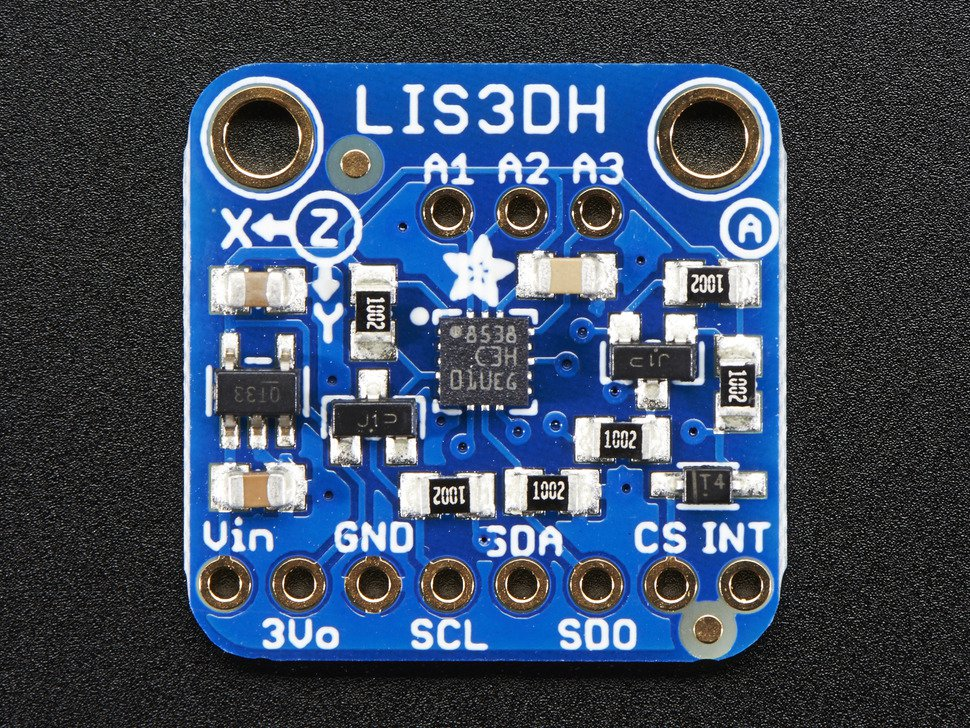
\includegraphics[width=\linewidth]{slike/lis3dh.jpg}
			\caption{Akcelerometar LIS3DH.}
			\label{fig:lis3dh}
		\end{figure}

		\par Ako se koristi I$^2$C, onda CS (\textit{Chip Select}) mora biti ili otpojen ili pritegnut na visoku naponsku razinu. U protivnom, ako se koristi SPI, onda CS mora biti pritegnut na masu.

		\par Sklop ima dvije moguće I$^2$C adrese - 0x18 i 0x19, tako da je moguće spojiti dva ovakva senzora na isti \textit{master}. Adresa se određuje tako da se pin SDO ostavi "u zraku" ili pritegne na nisku razinu za 0x18, odnosno na visoku razinu za 0x19. \\
		RPi3 u svojim GPIO pinovima ima dva para I$^2$C pinova - I$^2$C0 i I$^2$C1. Svejedno je koji se koristi, samo je, naravno, ključno da se parovi ne pomiješaju - SDA0 mora biti uparen s SCL0, a ne s SCL1, i obrnuto. Primjer I$^2$C spajanja prikazan je na Slici \ref{fig:lis3dhRpi} lijevo.

		\par Spajanje preko SPI-a izvodi se tako da je SCL i dalje u ulozi signala takta, ali je pin označen kao SDA sada u ulozi MOSI, a pin SDO u ulozi MISO pina. CS, kao što je već rečeno, za SPI mora biti uzemljen. Primjer SPI spajanja prikazan je na Slici \ref{fig:lis3dhRpi} desno.

		\begin{figure}[h!]
			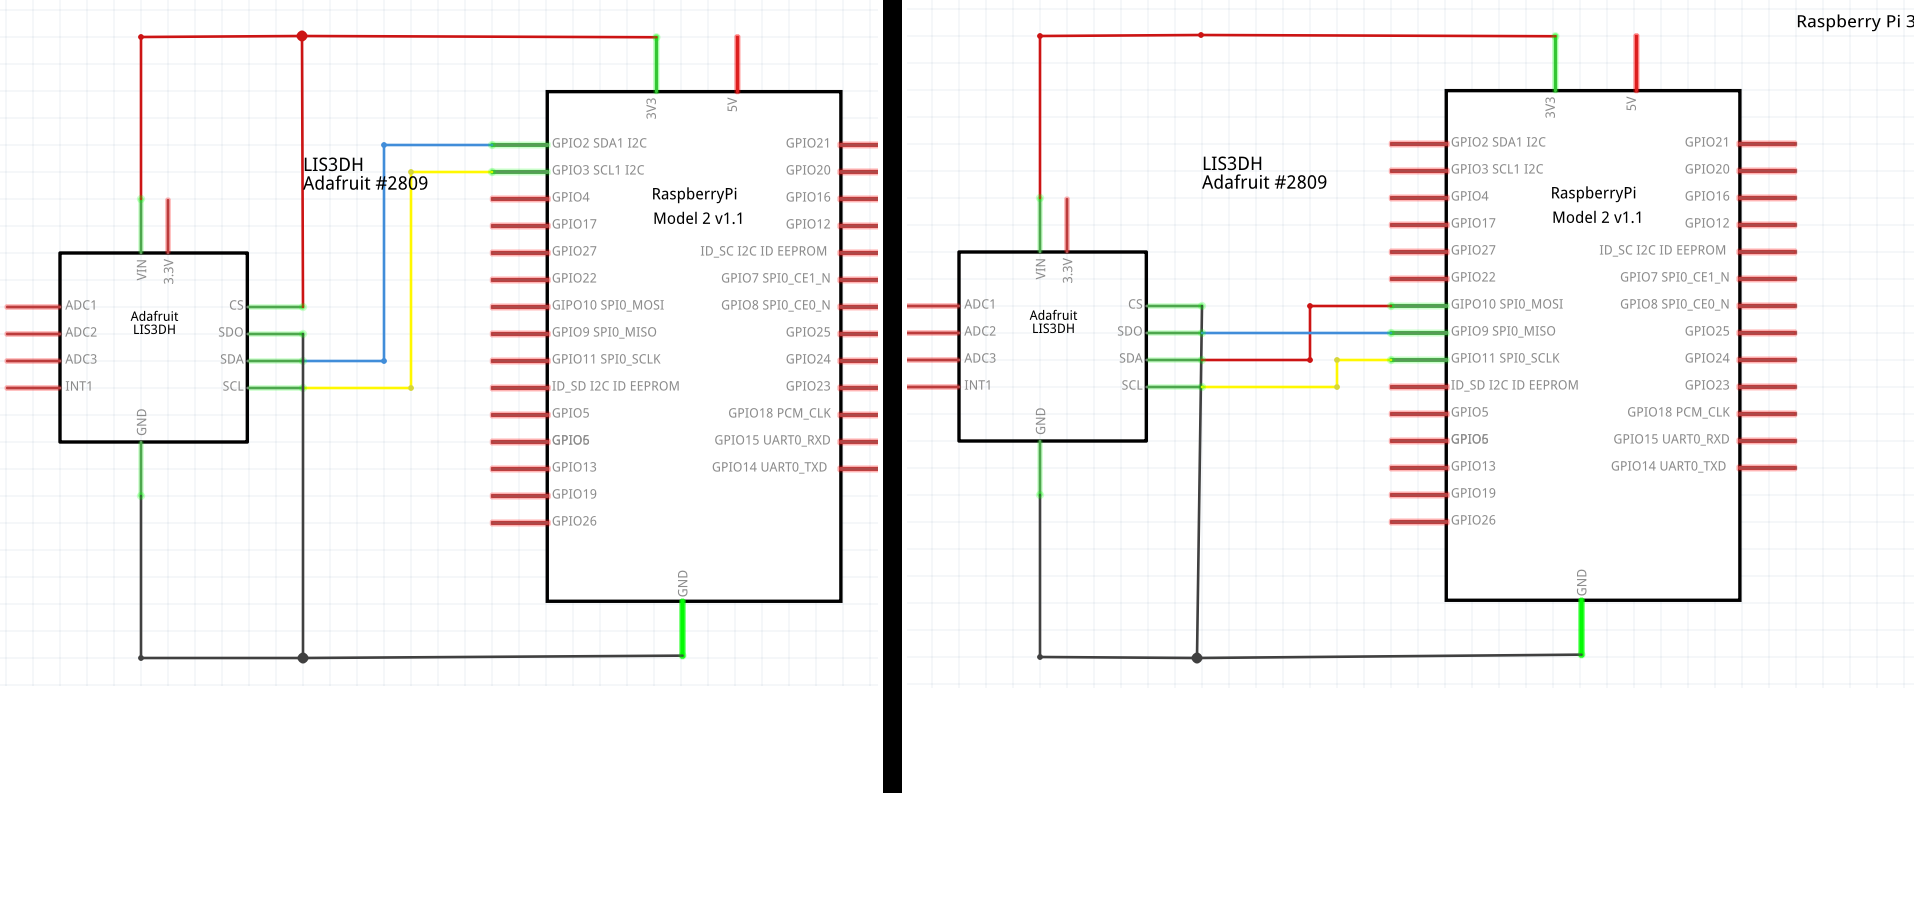
\includegraphics[width=\linewidth]{slike/i2cSpiMergeNoLabel.png}
			\caption{Primjer povezivanja LIS3DH i RPi3 - I$^2$C (lijevo) i SPI (desno).}
			\label{fig:lis3dhRpi}
		\end{figure}

		\par Ovime su ispunjeni sklopovski preduvjeti za osnovnu komunikaciju između senzora i RPi-ja, i za jednostavne primjere nije potrebno ništa više, ali ovaj senzor ima još nekoliko pinova koji nude interesantne mogućnosti:
		\begin{itemize}
			\item INT - \textbf{prekidni pin}
			\item A1, A2, A3 - analogno-digitalni pretvornici (engl. \textit{\textbf{ADC} - Analog-Digital Converter}) \\
		\end{itemize}

		Pinovi za ADC omogućuju da se na njih spoji neki analogni ulaz, koji će čip potom digitalizirati, s 10-bitnom preciznošću. Ovo se može pokazati pogodnim za situaciju u kojoj nemamo drugi ADC uređaj - kao što je, uostalom, i sâm RPi. RPi, naime, nema analogne, već samo digitalne ulaze, pa tako ADC pada u vodu bez dodatnog sklopovlja za tu namjenu.

		\par Prekidni pin omogućuje slanje prekidnog signala kao rezultat različitih događaja - senzor, naime, ima ugrađenu podršku za prepoznavanje jednostrukog i dvostrukog kuckanja, promjene orijentacije i slobodnog pada. Tu je podršku moguće iskoristiti kao okidač za generiranje prekida. Dakle, kada se dogodi neki događaj koji želimo pratiti (primjerice, kucanje po nekoj površini), sklop može generirati prekidni zahtjev da obavijesti RPi da je došlo do takvog događaja.




	\newpage
	\subsection{Mikrofon - Adafruit MAX4466}
		Drugi je senzor koji proučavamo također od tvrtke Adafruit, a riječ je o elektretskom mikrofonu. To je vrsta kondenzatorskog mikrofona koja princip rada temelji na električkim svojstvima materijala od kojeg je načinjen mikrofon - elektreta. Mikrofon je prikazan na Slici \ref{fig:max4466}.

		\begin{figure}[h!]
			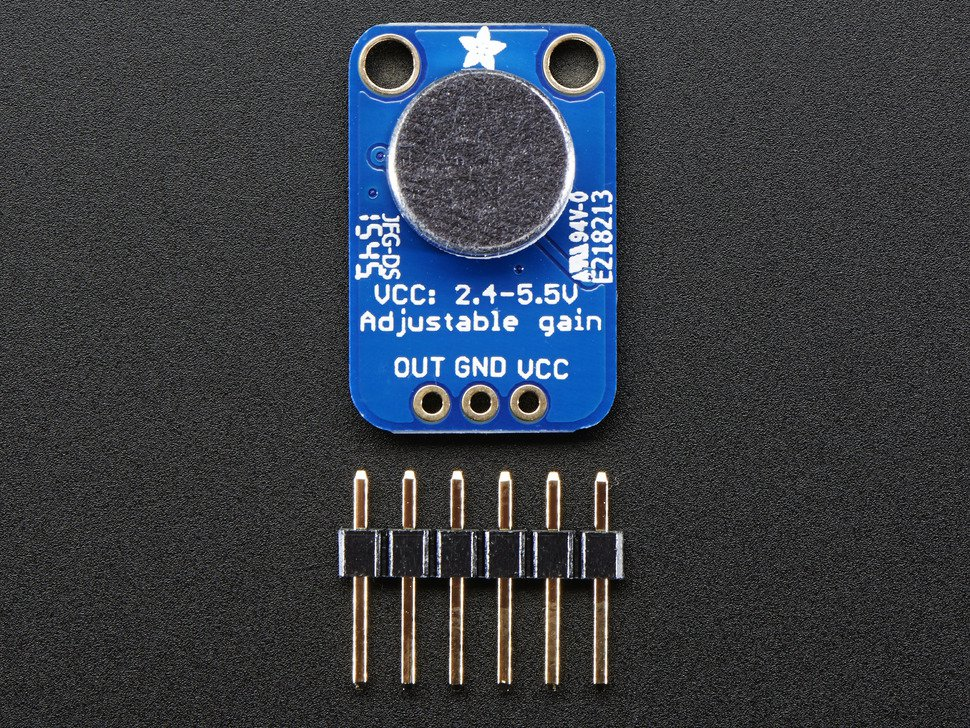
\includegraphics[width=\linewidth]{slike/4466.jpg}
			\caption{Adafruit MAX4466.}
			\label{fig:max4466}
		\end{figure}

		\par Sklop ima dva glavna funkcijska dijela:
		\begin{itemize}
			\item sâmi \textbf{elektretski mikrofon}, koji radi u rasponu frekvencija od 20Hz do 20kHz, i
			\item \textbf{operacijsko pojačalo Maxim MAX4466}, koje ima ugrađeno filtriranje šumova iz napajanja, što ga čini vrlo pogodnim za "čisto" pojačavanje mikrofonskog signala.
		\end{itemize}

		Sklop također nudi vrlo zgodnu mogućnost \textbf{sklopovski promjenjivog pojačanja} mikrofonskog signala, i to preko potenciometra koji se nalazi na stražnjoj strani sklopa, pa je tako faktor pojačanja moguće namjestiti na vrijednosti između 25 i 125. Ovo svojstvo omogućava širenje mogućnosti korištenja sklopa, jer ga je moguće prilagoditi i tihim i glasnim okruženjima.

		\par Budući da sklop ima samo 3 pina, za očekivati je da ga je relativno jednostavno koristiti - barem što se tiče spajanja. I doista - uz pinove GND i Vcc (uzemljenje, odnosno napajanje) postoji još samo pin OUT, na koji izlazi \textbf{analogni} signal. Što se tiče spajanja senzora na sklop koji "razumije" analogne signale, posao je završen. Ali - kao što je ranije napomenuto, RPi nema analogne, već samo digitalne ulaze, tako da je za očitavanje podataka sa senzora nužno u cijelu priču uvesti i neki ADC sklop. Ako bismo u istom projektu koristili i ranije obrađeni LIS3DH, koji ima 3 ADC ulaza, tada bismo jedan od tih analognih ulaza mogli upotrijebiti upravo za digitalizaciju izlaza mikrofona!

		\par Konačno, što se tiče električkih karakteristika sklopa, za njegovo je napajanje potrebno koristiti napon između 2.4 i 5V. Izlaz sklopa je istosmjerno spregnut (engl. \textit{DC coupled}), pa tako u potpuno tihom okruženju vrijednost na izlazu iznosi pola napona napajanja Vcc.


\section{Pregled dostupnih programskih okvira}
Tijekom pisanja ovog rada bio je dostupan samo akcelerometar LIS3DH, a budući da je taj senzor za kratku i jednostavnu demonstraciju rada sa senzorima bio i više nego dovoljan, LIS3DH je korišten za sva mjerenja prikazana u nastavku. Senzor će biti spojen na RPi koristeći protokol I$^2$C (kao što je prikazano na Slici \ref{fig:lis3dhRpi} lijevo), a za komunikaciju na programskoj razini koristit ćemo programski jezik \textbf{Python}, koji je vrlo pogodan upravo za brzu izradnju i testiranje prototipa različitih sustava.

\paragraph{\underline{GPIO komunikacija u Pythonu}} % (fold)
	\label{par:gpio_py}
		Kao što je rečeno, i Adafruit i Raspberry Pi Foundation su tvrtke otvorene filozofije poslovanja, pa nude gotove biblioteke funkcija za rad s njihovim proizvodima. Iako je Adafruitu matična platforma Arduino, postoji i službena biblioteka za korištenje GPIO sučelja s njihovim proizvodima u Pythonu. Budući da smo za korištenje akcelerometra predvidjeli koristiti I$^2$C, koji koristi određene GPIO pinove, svakako ćemo trebati tu biblioteku, dostupnu na Github repozitoriju: \url{https://github.com/adafruit/Adafruit_Python_GPIO}
		
	% paragraph gpio_py (end)

\paragraph{\underline{Biblioteka za LIS3DH}} % (fold)
	\label{par:lis3dh_lib}
		Sada kada imamo način komunikacije između Pythona i GPIO sučelja, potrebno je nekako uspostaviti komunikaciju i između GPIO sučelja i akcelerometra. Za taj će zadatak dobro poslužiti (neslužbena) biblioteka \texttt{python-lis3dh}, koja implementira glavnu funkcionalnost akcelerometra, a dostupna je na Github repozitoriju: \url{https://github.com/mattdy/python-lis3dh} \\
		Još vrijedi istaknuti da je u toj biblioteci implementirana i funkcija detekcije jednostrukog kucanja. Ostale funkcije (detekcija slobodnog pada i promjene orijentacije), nažalost, u ovoj biblioteci još nisu implementirane.


	% paragraph lis3dh_lib (end)

\paragraph{\underline{Programska podrška za MAX4466}} % (fold)
	\label{par:max4466_lib}
		Budući da MAX4466 ima analogni izlaz, a RPi samo digitalne ulaze, nekakva biblioteka funkcija za MAX4466 konceptualno jednostavno nije primjenjiv pojam. Budući da smo ionako primorani koristiti neki ADC sklop kao sučelje između RPi-ja i MAX4466, za očitavanje (digitaliziranog) izlaza MAX4466 poslužit će biblioteka za komunikaciju s GPIO pinovima, a jednom kada očitamo te podatke, njihova daljnja obrada ovisi o primjeni mikrofona.

	% paragraph max4466 (end)


\newpage
\section{Primjeri}
	Kao primjer korištenja akcelerometra provedeno je nekoliko relativno jednostavnih mjerenja:
	\begin{enumerate}
		\item Prvo je mjerenje provedeno tako da je senzor bio pričvršćen za vodoravnu površinu stola ljepljivom trakom - paralelno s njom - a promatrana su dva tipa podražaja:
		\begin{enumerate}
			\item \textbf{kucanje} po stolu uobičajene jačine
			\item \textbf{agresivno udaranje} šakom po stolu
		\end{enumerate}
		I kucanje i udaranje došlo je s druge strane stola - emulirajući, primjerice, kucanje na ulaznim vratima u stan. Također, svaki je period sadržao dva udarca, pa pauzu, a mjerena su 4 perioda. Svrha ovakvog mjerenja je utvrđivanje mogućnosti detekcije udarca na temelju \textbf{impulsne vibracije}. Radi lakšeg čitanja rezultantnog grafa i utvrđivanja preciznosti detekcije kucanja, ritam kucanja i udaranja pratio je metronom.
		\item Drugo je mjerenje provedeno tako da je senzor bio pričvršćen na tijelo bas gitare, te je potom \textbf{odsviran ton A} (približno 55 Hz). Ovo je mjerenje odrađeno sa svrhom utvrđivanja koliko dobro senzor "snima" \textbf{kontinuiranu vibraciju} (s prirodnim prigušenjem).
	\end{enumerate}

	Za prvo je mjerenje također korišten i \textbf{prekidni pin} (spojen na GPIO 04, što je definirano u datoteci \texttt{LIS3DH.py}), koji je generirao prekide kada bi otkrio kucanje.\\
	Budući da drugo mjerenje nije imalo impulsne podražaje, taj pin nije korišten. \\

	\par Za komunikaciju između laptopa i RPi-ja korišten je \textbf{SSH (Secure SHell) protokol}, koji omogućuje udaljeno upravljanje nekim računalom u mreži - u bitnome, omogućuje mrežni pristup terminalu OS-a na RPi-ju i pokretanje naredbi na njemu. \\

	Programski kôd i rezultati mjerenja (u grafičkom obliku) dani su u nastavku. \\

	\subsection{Programski kôd}

	\paragraph{\underline{Očitavanje podataka}} % (fold)
	\label{par:reading_data}
		Za testiranje senzora korišten je Python program iz navedenog repozitorija, čija je glavna funkcija izložena u nastavku:

		\lstinputlisting[style=Python]{testLIS3DH.py}

		\par Izlaz testnog programa se, dakle, većinski sastoji od ispisa \textbf{očitanja u X, Y i Z smjerovima}, a vrijednosti su realni brojevi, ugrubo u rasponu od -1 do 1. Radi sažetosti nije prikazan kôd odgovoran za otkrivanje kucanja, koje u ispis dodaje još nekoliko linija koje obavještavaju korisnika da je očitano kucanje ("single click").
		\par Program je, naravno, pokrenut na RPi-ju, \texttt{Bash} naredbom: \\
		\texttt {python testLIS3DH.py > out.txt}.

	% paragraph reading_data (end)

	\paragraph{\underline{Agregiranje i iscrtavanje rezultata}} % (fold)
	\label{par:plotting}
		Da bismo na temelju očitanih podataka mogli iscrtati grafove, izlaz mjerenja spremljen je u tekstualnu datoteku \texttt{out.txt} na RPi-ju. Koristeći \textbf{SCP (Secure Copy Protocol)}, protokol za kopiranje datoteka između računala u mreži, ta je datoteka potom prebačena na laptop, gdje su podaci agregirani i vizualizirani. Za to je poslužila jednostavna Bash skripta:

		\lstinputlisting[style=Bash]{prepare.sh}

		\par Dakle, nakon prebacivanja datoteke s očitanjem na laptop (prva linija skripte) i njenog uređivanja (uklanjanje početnih linija koje ne sadrže mjerene podatke; druga linija skripte), u trećoj je liniji pokrenut vlastiti Python program koji agregira podatke i, koristeći ugrađenu biblioteku \textbf{\texttt{matplotlib.pyplot}}, iscrtava ih na grafove. Ukupno su generirane 4 za mjerenje impulsa, odnosno 3 krivulje za mjerenje kontinuirane vibracije:

		\lstinputlisting[style=Python]{plotter.py}

	% paragraph plotting (end)


	Nije zgorega napomenuti da je bilo potrebno malo modificirati postojeći programski kôd kako bi proradio, jer je Adafruit repozitorij promijenjen od zadnje verzije \texttt{python-lis3dh} biblioteke. Promjene se odnose na datoteku \texttt{LIS3DH.py} iz biblioteke \texttt{python-lis3dh}:
		\begin{itemize}
			\item Linija koja se odnosi na učitavanje I$^2$C podrške više nije 
			\texttt{from Adafruit\_I2C import Adafruit\_I2C} jer je \texttt{Adafruit\_I2C} verzija te biblioteke koja se više ne koristi. Sada je uputno koristiti biblioteku \texttt{Adafruit\_GPIO.I2C}, pa taj \textit{import} izgleda ovako:
			\texttt{import Adafruit\_GPIO.I2C as I2C}. 
			Nakon što su načinjene te promjene, u tijelu biblioteke još je potrebno izmijeniti svako pojavljivanje zastarjelog objekta \texttt{Adafruit\_I2C} u aktualni \texttt{I2C.Device}.
			\item Konstruktor klase \texttt{LIS3DH} za pretpostavljenu oznaku I$^2$C sabirnice koristi vrijednost "-1", dok RPi ima samo sabirnice s oznakama "0" i "1". Prema tome, ovisno o tome koja se od njih koristi (u nastavku rada je to sabirnica 1), potrebno je ili "hardkodirati" vrijednost sabirnice ili naći način za detekciju korištene sabirnice. Zbog vremenskih ograničenja i obujma ovog rada, prihvatljivo je rješenje bilo "hardkodirati" vrijednost "1", pa tako zaglavlje konstruktora klase \texttt{LIS3DH} izgleda ovako: \\ 
			\texttt{def \_\_init\_\_(self, address=0x18, \underline{bus=1}, debug=False)}.
		\end{itemize}
		Nakon ovih preinaka, biblioteka je postala funkcionalna.

	\newpage
	\subsection{Očitani podaci}
	Preostaje nam još proučiti dobivene grafove. Na svim grafovima vrijedi sljedeća legenda:
	\begin{itemize}
		\item Crvena boja - X os akcelerometra,
		\item Zelena boja - Y os akcelerometra,
		\item Plava boja - Z os akcelerometra,
		\item Crna boja - detekcija kucanja.
	\end{itemize}

	\paragraph{\underline{Kucanje}} % (fold)
	\label{par:click}
	Prvo je na redu kucanje. Prikazano je grafom na Slici \ref{fig:click}.

	\begin{figure}[h!]
	  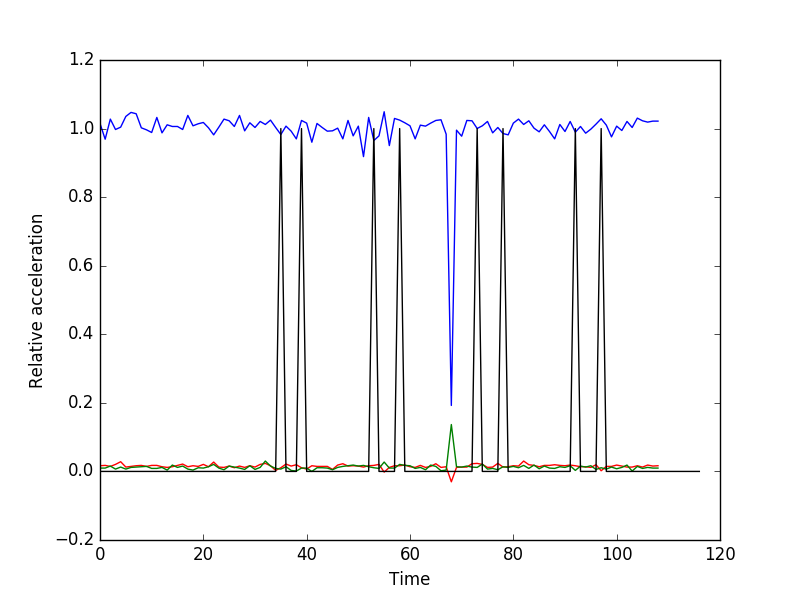
\includegraphics[width=\linewidth]{slike/click.png}
	  \caption{Kucanje}
	  \label{fig:click}
	\end{figure}

	Odmah je očito da specijalizirana detekcija kucanja radi ispravno - vide se 4 para kucanja. Međutim, interesantno je da se, barem "na prvu", kucanje ne može intuitivno iščitati iz valnog oblika nijedne od krivulja. Z-os ima najveće oscilacije, što i ima smisla, jer je akcelerometar bio učvršćen vodoravno i prema gore (zato vrijednosti za Z os osciliraju oko 1, a ne oko 0 kao što je to slučaj za preostale dvije osi), pa je svaki udarac najviše utjecao upravo na nagib senzora.
	\par Dobro je primijetiti i da su već u takvom, relativno slabo učvršćenom okruženju, šumovi i slabe okolne vibracije, dovoljno prigušeni za X i Y osi. Izvor artefakta na cca. 65. vremenskoj jedinici nije poznat, ali interesantno je primijetiti da ni takva velika anomalija nije uspjela "zbuniti" sustav za detekciju kucanja.

	% paragraph click (end)
	\newpage
	\paragraph{\underline{Udaranje}} % (fold)
	\label{par:aggro}
	Sljedeći graf koji promatramo jest udaranje. Prikazan je na Slici \ref{fig:aggro}.

	\begin{figure}[h!]
	  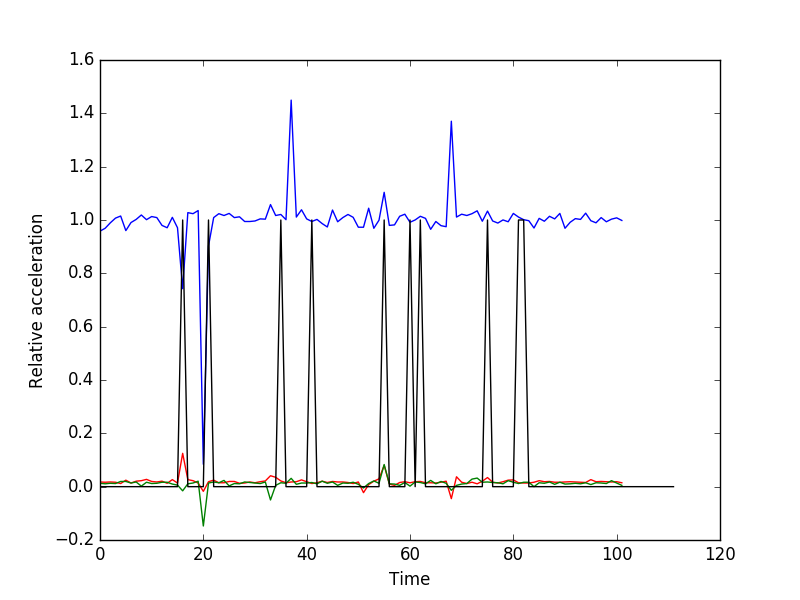
\includegraphics[width=\linewidth]{slike/aggro.png}
	  \caption{Udaranje}
	  \label{fig:aggro}
	\end{figure}

	U ovom slučaju detekcija kucanja također uglavnom radi - prvi i drugi par udaraca izgledaju kako bi trebali izgledati. Međutim, na trećem je paru senzor očitao i jedan lažni udarac, dok je zadnji udarac izazvao za senzor toliko snažne vibracije da je nekoliko vremenskih jedinica bio postavljen prekidni signal, što rezultira valnim oblikom koji nema "špicu", nego traje neko vrijeme.
	\par Također, na ovom se grafu već \textit{nešto} može zaključiti i na temelju valnih oblika pojedinih osi. Ipak, očito i dalje takav pristup nije sasvim pouzdan. Možemo zaključiti da sklop snažne udarce ne podnosi najbolje što se tiče preciznosti mjerenja, ali to je možda i adekvatno za sustav gdje je poželjna visoka osjetljivost - u mirnim periodima sklop ne oscilira jako, pa bi se, uz propisno učvršćivanje i eliminaciju šuma, mogao jako dobro iskoristiti.

	% paragraph aggro (end)

	\newpage
	\paragraph{\underline{Prigušeno titranje}} % (fold)
	\label{par:bass}
	Posljednji graf predstavlja "snimku" tona A odsviranom na električnoj bas gitari. Graf je prikazan na Slici \ref{fig:bass3}.

	\begin{figure}[h!]
	  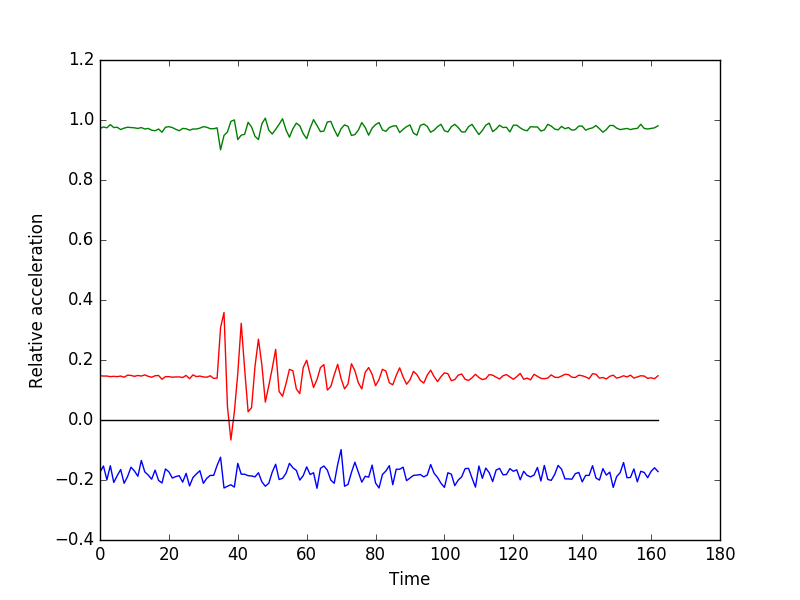
\includegraphics[width=\linewidth]{slike/bass3.png}
	  \caption{Ton A}
	  \label{fig:bass3}
	\end{figure}

	Čim pogledamo valni oblik na X-osi, očito da je senzor očitao nekakvo prigušeno titranje ugrubo stalne frekvencije. Na Z-osi i dalje vidimo najveći šum, iz istog razloga kao i ranije. Y-os, pak, opet ima prilično malen šum, pogotovo prije trenutka 40. Oko trenutka 40 je trznuta žica, te instrument počinje vibrirati - na X-osi vidimo da je riječ o stabilnoj frekvenciji i urednom prigušenju. Titranje je daleko najizraženije na X-osi zato što je pravac titranja žice skoro potpuno poklopljen s tom osi, pa se svaki titraj daleko najviše osjeti na dijelu sklopa zaduženom za očitanje na toj osi.
	\par Iz ovog eksperimenta možemo zaključiti da LIS3DH, iako je akcelerometar, a ne mikrofon, pa vrlo vjerojatno nije optimiziran za stabilno očitanje frekvencije, pokazuje sasvim pristojne i predvidive rezultate u okruženju s kontinuiranom vibracijom. Bilo bi interesantno ponoviti eksperiment i s mikrofonom MAX4466, pa usporediti rezultate, ali, nažalost, taj mikrofon trenutno nije na raspolaganju.

	% paragraph bass (end)


\newpage
\section{Zaključak}
	Cilj ovog rada bio je izložiti kratak opis računala Raspberry Pi, te demonstrirati široke mogućnosti njegovog korištenja s različitim senzorima. Iz svega navedenog, može se zaključiti da je RPi3 jedan iznimno fleksibilan sklop, koji je interesantan mnogim entuzijastima i stručnjacima - poglavito zbog ogromnog spektra mogućnosti koje nudi, kako u \textit{low-level} ugradbenoj, tako i u IoT (\textit{Internet of Things}, koncepcija spajanja ugradbenog sklopovlja na internet) domeni. Računalo je kao takvo vrlo popularno u raznim kućnim projektima, poput automatizacije nekih zadataka ili praćenja kontinuiranih prilika (poput, primjerice, temperature, buke ili kretanja), a vrlo je iskoristiv i u multimedijske svrhe. \\

	\par Ma koliko RPi bio moćan, ipak je i dalje riječ o ugradbenom računalu, pa je razumno očekivati da ima podršku za \textit{low-level} komunikaciju. Naravno, to je očekivanje ispunjeno - najpopularniji sklopovski komunikacijski protokoli (SPI, I$^2$C i TTL) su podržani i u potpunosti implementirani. Naravno, nije se stalo tu - implementirana je i podrška za USB i internetsku vezu, a od inačice 3 postoji i sasvim stabilna podrška za bežičnu vezu - konkretno, za \textit{WiFi} i \textit{Bluetooth} protokole. \\

	\par Uz RPi, izloženi su i jedan akcelerometar (LIS3DH) i jedan mikrofon (MAX4466), s posebnim osvrtom na njihovu komunikaciju s RPi-jem. Riječ je o interesantnim sklopovima koji pružaju mnogo mogućnosti, a iznimno ih je jednostavno "upregnuti" uz RPi. \\

	\par Budući da je riječ o otvorenim tehnologijama, ne čudi da je na internetu dostupno mnoštvo gotovih i funkcionalnih biblioteka za korištenje i računala i senzora, a te se biblioteke još uvijek razvijaju i otvorene su za korištenje i suradnju svim entuzijastima. Za LIS3DH je obavljeno i nekoliko eksperimenata u kojima se mjerio odziv senzora na različite podražaje. Izloženi su i prokomentirani rezultati mjerenja, i pokazalo se da je za dobar dio primjena LIS3DH ponudio vrlo dobre rezultate. Možda nije sasvim adekvatan za neka vrlo precizna mjerenja, ali je svakako dovoljno osjetljiv za većinu primjena. \\

	\par Sve u svemu, RPi3 je vrlo moćan stroj koji je donio revoluciju u ugradbene sustave, a svakako je - zbog jednostavnosti primjene, spektru mogućnosti i raširenosti programske podrške, a i intelektualnih izazova koje nudi - našao svoje mjesto u okruženjima za edukaciju i prototipe.


\newpage
\section{Literatura}

\begin{itemize}
	\item Raspberry Pi službene stranice: \url{https://www.raspberrypi.org/}
	\item LIS3DH: \url{https://learn.adafruit.com/adafruit-lis3dh-triple-axis-accelerometer-breakout/downloads?view=all}
	\item MAX4466: \url{https://www.adafruit.com/product/1063}
	\item Korištenje I$^2$C sučelja kroz Python: \url{http://www.instructables.com/id/Raspberry-Pi-I2C-Python/}
\end{itemize}

\end{document}
